\chapter{Design}
This chapter of the report has the purpose of presenting the architecture of the DC-Net simulator from different perspectives through the utilization of UML diagram notations. The overview of the system is still an abstract one, but it is an important step to realize a successful implementation. 

Firstly, the architecture diagrams of the application and examples of the event-based communication will be shown. Following, there is a series of sequence diagrams that exemplifies the data flow between clients and server both for the basic implementation of the protocol and the advanced one.


\section{System Architecture}
The architecture of the simulator is simple.  


\section{Minimal Distributed Architecture}



\section{Event-Based Communication Example}
View from single client point of view.



\section{Basic Data Flow Design}


\section{Advanced Data Flow Design}



\begin{figure}[h!]
    \centering
    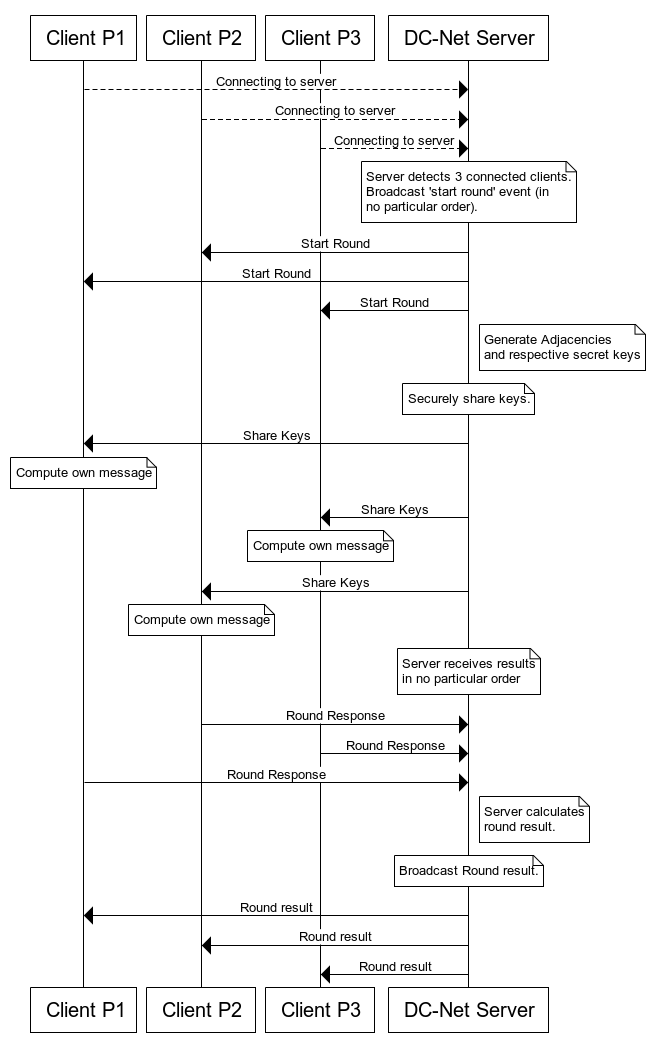
\includegraphics[width=0.8\textwidth]{Images/successfulRound.png}
    \caption{Successful Round of communication.}
    \label{fig:useCaseSuccessfulRound}
\end{figure}
